\documentclass{article}
\usepackage{float}
\usepackage{amsmath}
\usepackage{amssymb}
\usepackage{enumitem}
\usepackage{geometry}
\usepackage{verbatim}
\usepackage{graphicx}  % Package to handle images
\usepackage{hyperref}
\geometry{a4paper, margin=1in}

\title{Assignment 1 \\ Machine Learning}
\author{Mohammad Hossein Basouli - 401222020}
\date{}

\begin{document}

\maketitle

\section*{Theoretical Questions}
\subsection*{Exercise 1}
First, we assume that we are using \( z \) and \( t \) - tests for estimating the population mean.

\subsubsection*{Assumptions}
\begin{itemize}
    \item The \( z \)-test assumes that:
    \begin{itemize}
        \item The sample size is large (\( n > 30 \)).
        \item Samples are chosen independently.
        \item The population standard deviation is known.
        \item The sample mean follows a normal distribution.
    \end{itemize}
    \item The \( t \)-test assumes that:
    \begin{itemize}
        \item The sample size does not need to be large.
        \item Samples are chosen independently.
        \item The population variance is unknown.
        \item The statistic \( \frac{\overline{x} - \mu}{\frac{s}{\sqrt{n}}} \) follows a \( t \)-distribution.
    \end{itemize}
\end{itemize}

\subsubsection*{Population Standard Deviation}
We discussed this earlier.

\subsubsection*{Use Cases}
\begin{itemize}
    \item \( z \)-test:
    \begin{itemize}
        \item Used to check whether the sample mean differs significantly from the population mean when the population variance is known.
        \item Used to check whether two populations differ significantly in their means when the variances of both populations are known.
    \end{itemize}
    \item \( t \)-test:
    \begin{itemize}
        \item Used to check whether the sample mean differs significantly from the population mean when the population variance is unknown.
        \item Used to check whether two populations differ significantly in their means when the variances of both populations are unknown.
    \end{itemize}
\end{itemize}

\subsection*{Exercise 2}
As n goes beyond 30, from the Central Limit Theorem (CLT), we can say:

\[
P(4.5 \leq \bar{X}) = P\left( \frac{4.5 - 4.2}{\frac{0.5}{\sqrt{30}}} \leq \frac{\bar{X} - \mu}{\frac{\sigma}{\sqrt{n}}} \right)
\]

\[
= P\left( \frac{0.3 \times \sqrt{30}}{0.5} \leq Z \right) = 0.00051904
\]

\subsection*{Exercise 3}

\subsubsection*{Scenario a)}
We apply Pearson's correlation test to determine whether there is a linear relationship between Age and Annual Income. Pearson's correlation is the most suitable test for detecting linear relationships:
\[
\text{correlation} = \frac{\sum_i (x_i - \overline{x}) (y_i - \overline{y})}{(n - 1) \sigma_x \sigma_y}
\]
\[
r \approx 0.98
\]
\[
\text{Correlation test: } t = r\sqrt{\frac{n-2}{1-r^2}}
\]
\[
p\text{-value} \approx 0.0035 < 0.05
\]

\subsubsection*{Scenario b)}
for monotonic relationships but not necessarily linear, Spearman's correlation test is the most appropriate:
\[
\text{Spearman correlation} = \frac{\text{Cov}(R[x], R[y])}{\sigma_{R[x]} \cdot \sigma_{R[y]}}
\]
\[
r = -0.9
\]
\[
\text{Spearman correlation test}
\]
\[
p\text{-value} = 0.037 < 0.05
\]

\subsection*{Exercise 4}
\begin{itemize}
    \item Key difference: The Mann-Whitney U test is used for comparing two independent samples, whereas the Wilcoxon signed-rank test is used for paired samples.
    \item Conclusion: We use the Mann-Whitney U test because the strategies being compared are independent.
\end{itemize}

\subsection*{Exercise 5}
\begin{enumerate}[label= \alph*]
    \item We need to answer two questions:
    \begin{enumerate}
        \item Are the residuals within each group normally distributed? In this case, they are, since the Shapiro-Wilk test yields a \( p \)-value of \( 0.43 > 0.05 \).
        \item Is the variance equal across groups? According to Levene's test, the \( p \)-value is \( 0.86 > 0.05 \), indicating homogeneity of variance.
    \end{enumerate}
    Conclusion: Since both assumptions for ANOVA are met, we can perform the test. The ANOVA test gives a \( p \)-value of \( 1.4 \times 10^{-9} \), suggesting a significant difference between groups in terms of "Feature X".
    
    \item The results from part (a) confirm a significant difference between groups based on the p-value.
    
    \item The MANOVA test could be used to examine whether there are significant differences between groups across multiple dependent variables.
    
    \item If at least one feature contributes significantly, we can decide between ANOVA and the Kruskal-Wallis test. Each variable must be analyzed separately to determine if it significantly differentiates the groups. If it does, it can be considered as a feature.
\end{enumerate}

\section*{Practical Questions}

\subsection*{Sleep Health}
\begin{enumerate}
    \item \textbf{Exploratory Data Analysis (EDA)}:
    
    \begin{itemize}

        \item \textbf{Number of rows (data samples) and columns (features) are in the dataset}: (374, 13)
     
        \item \textbf{Values for each categorical feature}:
        \begin{itemize}

            \item \textbf{Gender}:
            \begin{verbatim}

                ['Male' 'Female']

            \end{verbatim}

            \item \textbf{Occupation}:
            \begin{verbatim}

                ['Software Engineer' 'Doctor' 'Sales Representative' 'Teacher' 'Nurse'
                'Engineer' 'Accountant' 'Scientist' 'Lawyer' 'Salesperson' 'Manager']

            \end{verbatim}

            \item \textbf{BMI Category}:
            \begin{verbatim}

                ['Overweight' 'Normal' 'Obese' 'Normal Weight']

            \end{verbatim}

            \item \textbf{Sleep Disorder}:
            \begin{verbatim}

                [NaN 'Sleep Apnea' 'Insomnia']

            \end{verbatim}

        \end{itemize}

        \newpage
        \item \textbf{Description of numerical features}:
        \begin{figure}[H]  % 'h' means place the figure here

            \centering
            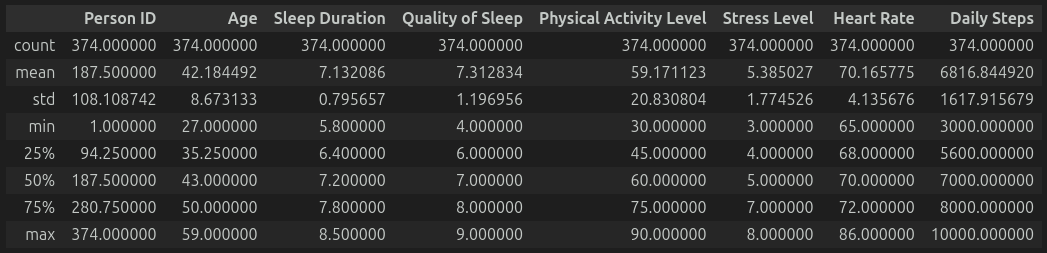
\includegraphics[width=0.8\textwidth]{./images/health_description_of_numeric_columns.png}  % Adjust width as needed
            \caption{Description of numerical features}
            \label{fig:Figure_1}  % Reference the figure using \ref{fig:sample}
        \end{figure}

        \item \textbf{Datatype of each feature}:
        \begin{verbatim}

            #   Column                   Non-Null Count  Dtype  
            ---  ------                   --------------  -----  
             0   Person ID                374 non-null    int64  
             1   Gender                   374 non-null    object 
             2   Age                      374 non-null    int64  
             3   Occupation               374 non-null    object 
             4   Sleep Duration           374 non-null    float64
             5   Quality of Sleep         374 non-null    int64  
             6   Physical Activity Level  374 non-null    int64  
             7   Stress Level             374 non-null    int64  
             8   BMI Category             374 non-null    object 
             9   Blood Pressure           374 non-null    object 
             10  Heart Rate               374 non-null    int64  
             11  Daily Steps              374 non-null    int64  
             12  Sleep Disorder           155 non-null    object 
            dtypes: float64(1), int64(7), object(5)

        \end{verbatim}

        \item \textbf{Data pre-processing}:
        \begin{itemize}
            
            \item We begin Data pre-processing, by first looking at what columns have NaN entries in them and how many there are:
            \textit{From the last bullet, we can see that 374 - 155 = 219 entries in the column, 'Sleep Disorder' are filled with NaN, and the are the only NaN entries in our dataset.} 
            \item Next, we divide the dataset into three different groups, according to the range of values that features 'Sleep Disorder' can take on, including NaN values. If we plot the distribution of all of the features for each of the groups, 
            we would end up with something like Figure~\ref{fig:Figure_2}:
             
            \begin{figure}[H]  % 'h' means place the figure here

                \centering
                \includegraphics[width=0.8\textwidth]{./images/health_dpp_comparison_of_columns.png}  % Adjust width as needed
                \caption{Plot of features for each of the groups (zoom-in)}
                \label{fig:Figure_2}  % Reference the figure using \ref{fig:sample}
    
            \end{figure}
            \item Figure~\ref{fig:Figure_2} roughly shows that, people with NaN value in the column 'Sleep Disorder' are people who don't have any Sleep Disorder and are healthy and OK.
            \item Some of the arguments that would lead us to this conclusion that people with NaN values don't have any Sleep Disorder are as follows:
            \begin{enumerate}
                \item They roughly have an even distribution of 'Sleep Duration' over the range between 7 and 8 hours. Which makes sense, because healthy people have a similar distribution of Sleep Duration as well.
                \item Most of the them (\~80\%), have Normal BMI.
                \item They roughly have an even distribution of 'Heart Rate' over the range between 65 and 75. Which matches with what we would expect from healthy people.
                \item They also have an even distribution of 'Stress Level', and their distribution is not skew to one direction. which makes sense for normal people.
            \end{enumerate} 
        
        \end{itemize}
        
    \end{itemize}

    \item \textbf{Hypothesis Testing}:
    \begin{enumerate}[label=(\alph*)]

        \item Does women's sleep duration follow a normal distribution?
        \begin{itemize}
            \item Answer based on visualization (Figure~\ref{fig:Figure_3}):
            \textit{No, it doesn't seem to be normally distributed}
            \begin{figure}[H]  % 'h' means place the figure here

                \centering
                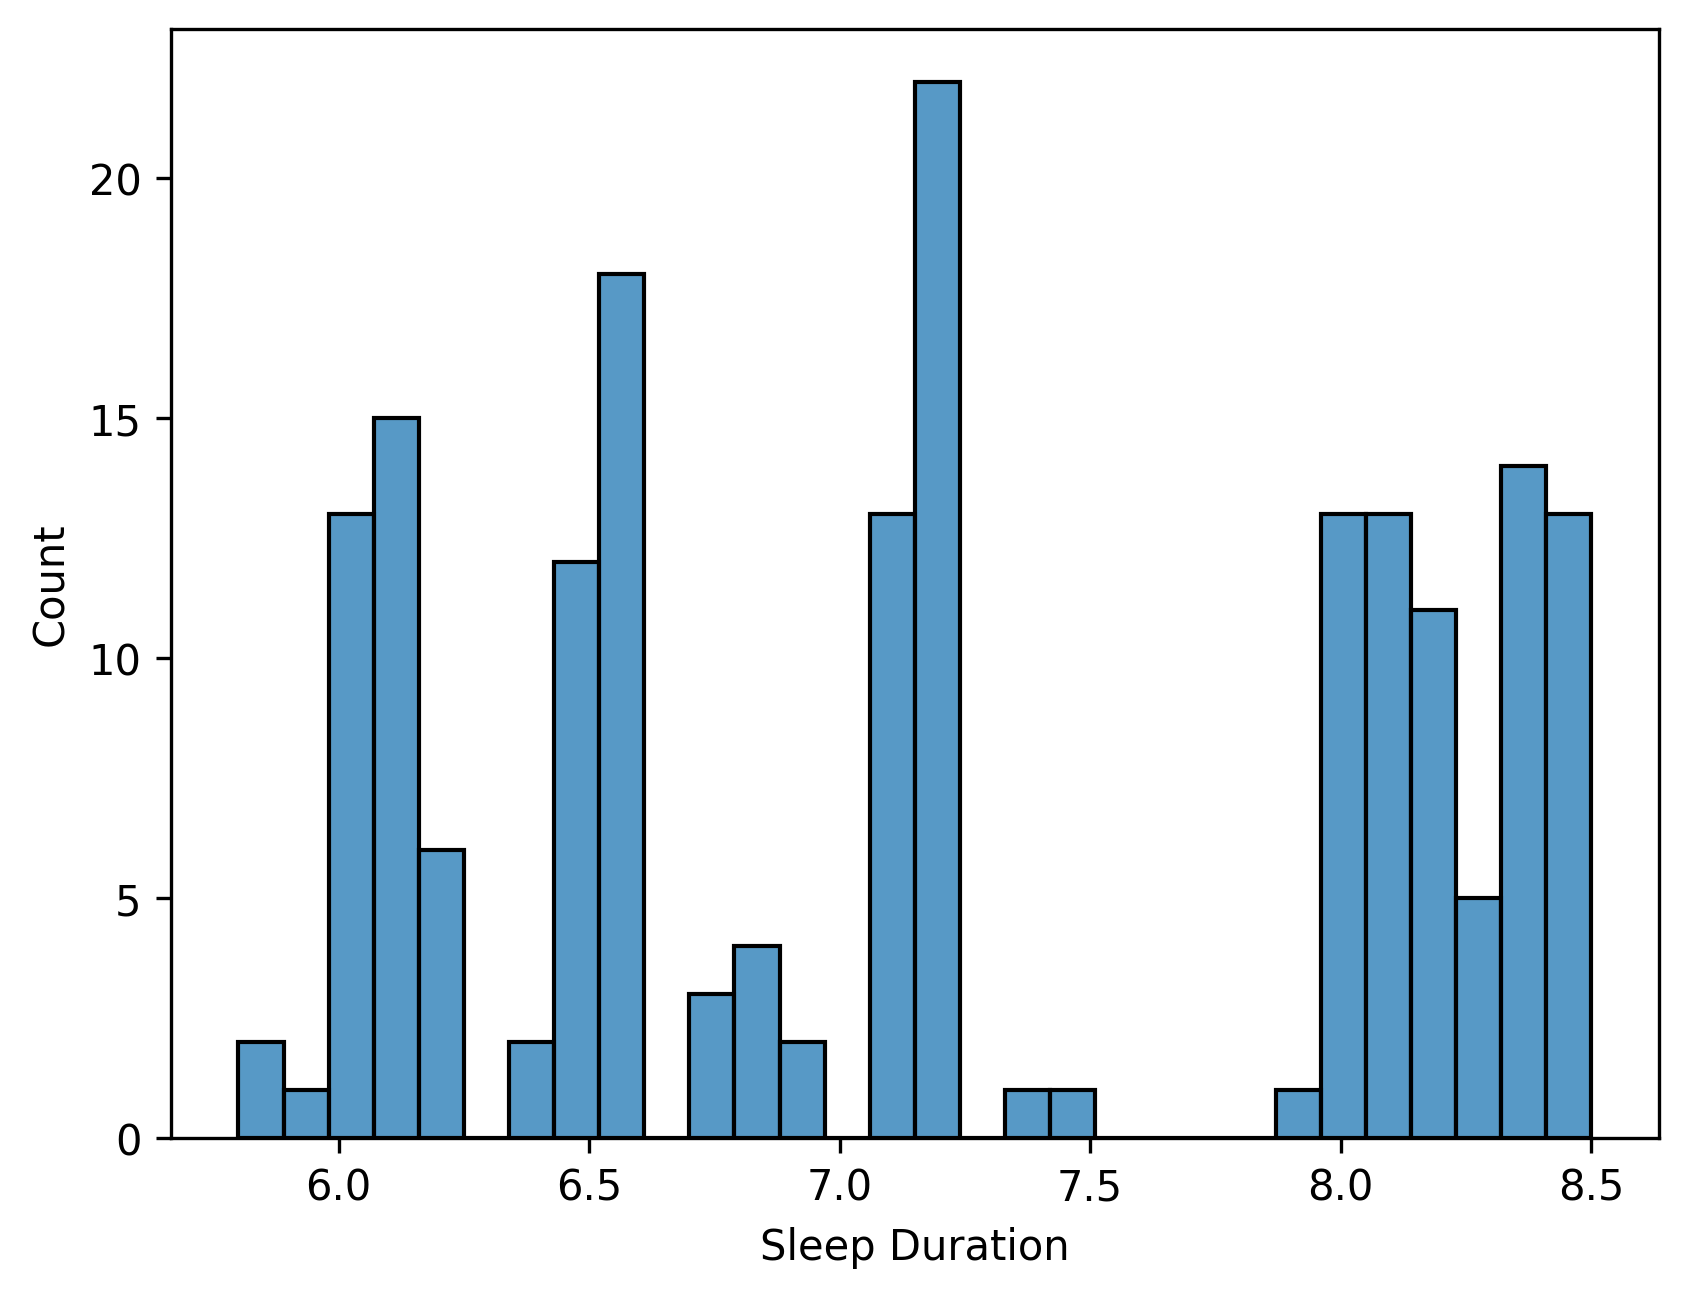
\includegraphics[width=0.8\textwidth]{./images/health_distribution_of_sleep_duration_women.png}  % Adjust width as needed
                \caption{Disribution of \textbf{Sleep Duration} for Women}
                \label{fig:Figure_3}  % Reference the figure using \ref{fig:sample}
    
            \end{figure}
            
            \item Answer based on hypothesis test:
            \textit{No, the p-value is so small, so we reject hypothesis that distribution is normal.}

        \end{itemize}

        \item Is having higher daily steps a contributing factor into better sleep? Check the corresponding correlation of Daily Steps and Quality of Sleep.
        \begin{itemize}
            \item First, we have to check to see what correlation test have to use for these two variables.
            \begin{itemize}
                \item If we look at the scatter plot of these two variables, we can see that the relationship between these two variables is not linear; So we head over to the Spearman Correlation test.
                \begin{figure}[H]  % 'h' means place the figure here

                    \centering
                    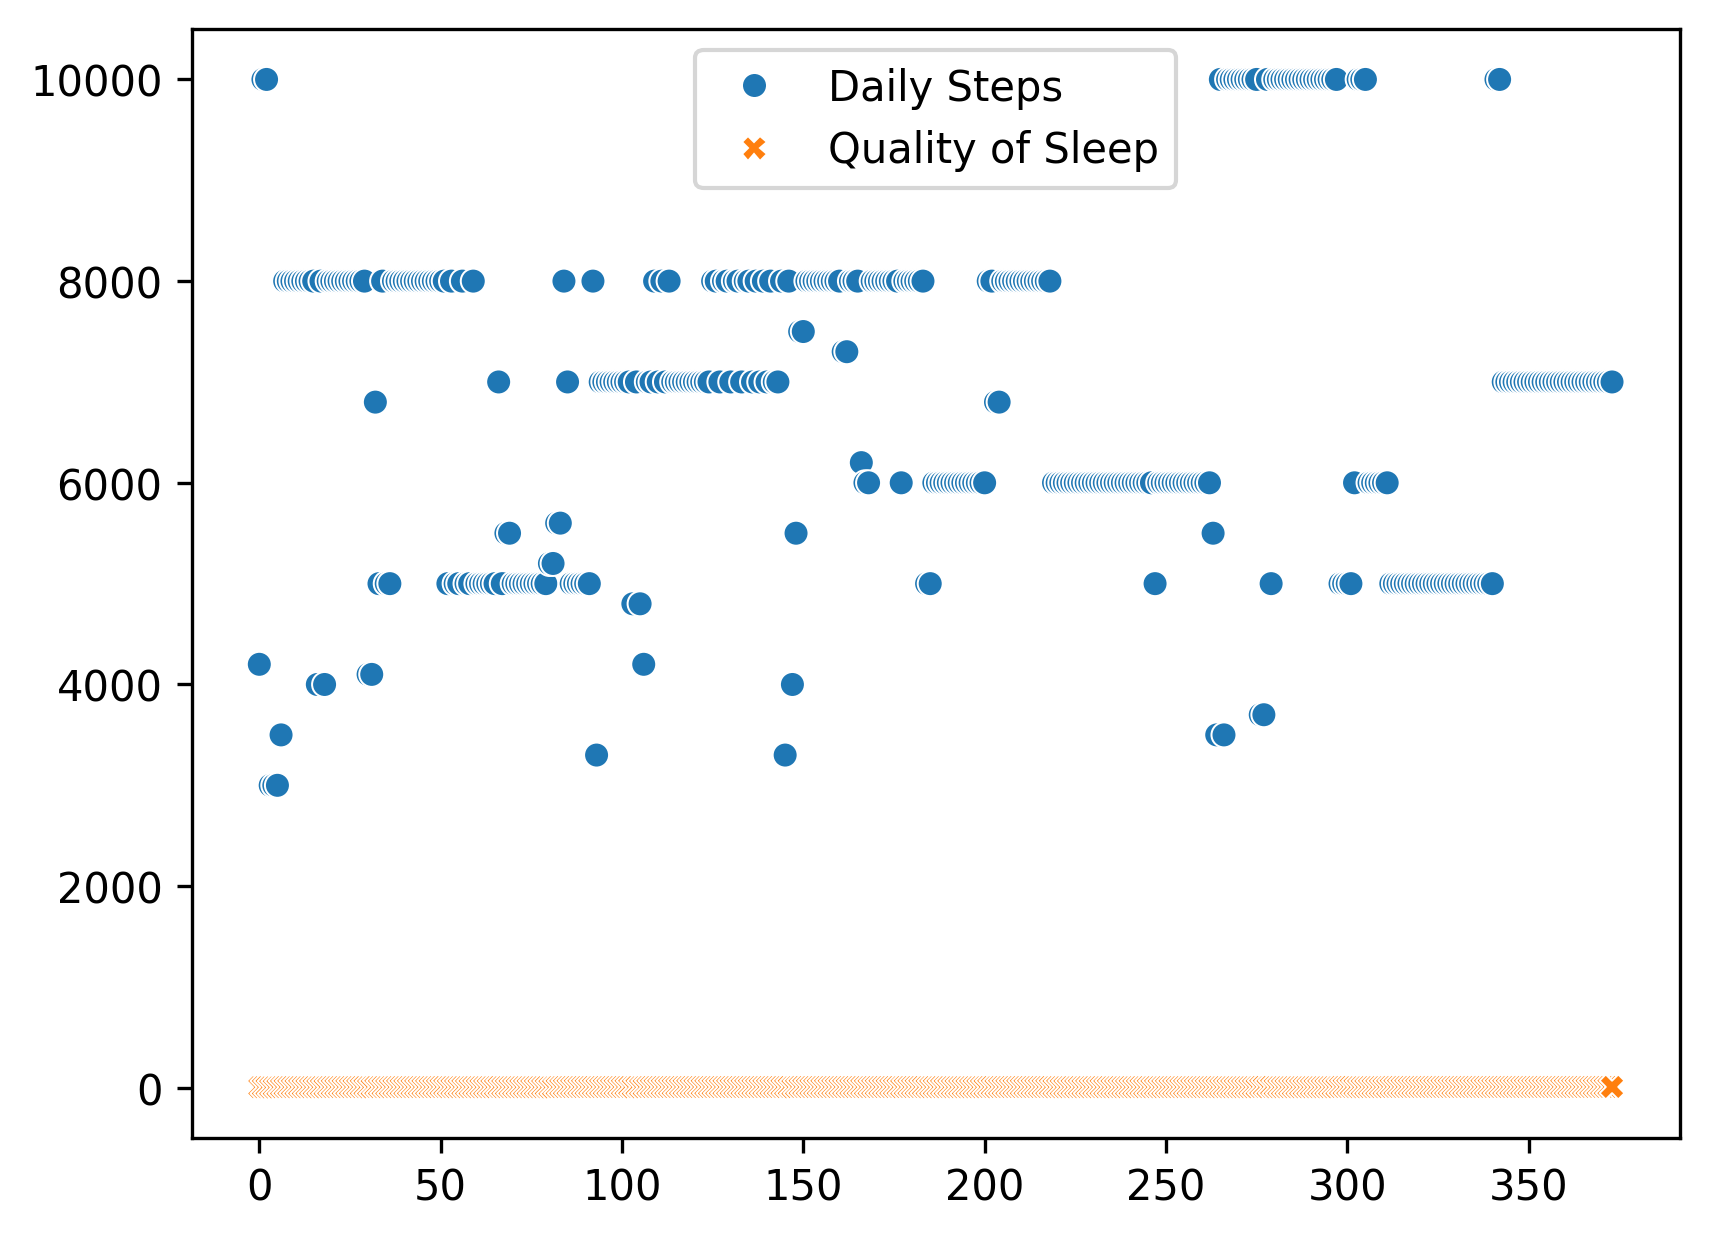
\includegraphics[width=0.8\textwidth]{./images/health_scatter_plot_of_daily_steps_quality_of_sleep.png}  % Adjust width as needed
                    \caption{Scatter plot of two variables, \textbf{Daily Steps and Quality of Sleep}}
                    \label{fig:Figure_4}  % Reference the figure using \ref{fig:sample}
        
                \end{figure}
            \end{itemize}

            \item If we run Spearman Correlation test, we would get the following result: Spearman Correlation Coefficient: 0.022779213378418182, P-value: 0.6605808344543287. Which shows that, there is no significant correlation between these two features. 
        \end{itemize}

        \item Is stress level different among different occupations? First, check this
        hypothesis with a test, and then compute the average stress level among
        different occupations. Use a bar chart or any other desired visualization
        method to demonstrate the result.
        \begin{itemize}
            \item Answer based on visualization (Figure~\ref{fig:Figure_5}):
            \textit{Yes, it really seems like that we have a significant difference in \textbf{stress level} in terms of different \textbf{Occupations}. e.g. we can easily see that stress level of salespersons is only distributed around 7 which is really high, but the stress level of most of the engineers is about 3 which is really low.}
            \begin{figure}[H]  % 'h' means place the figure here

                \centering
                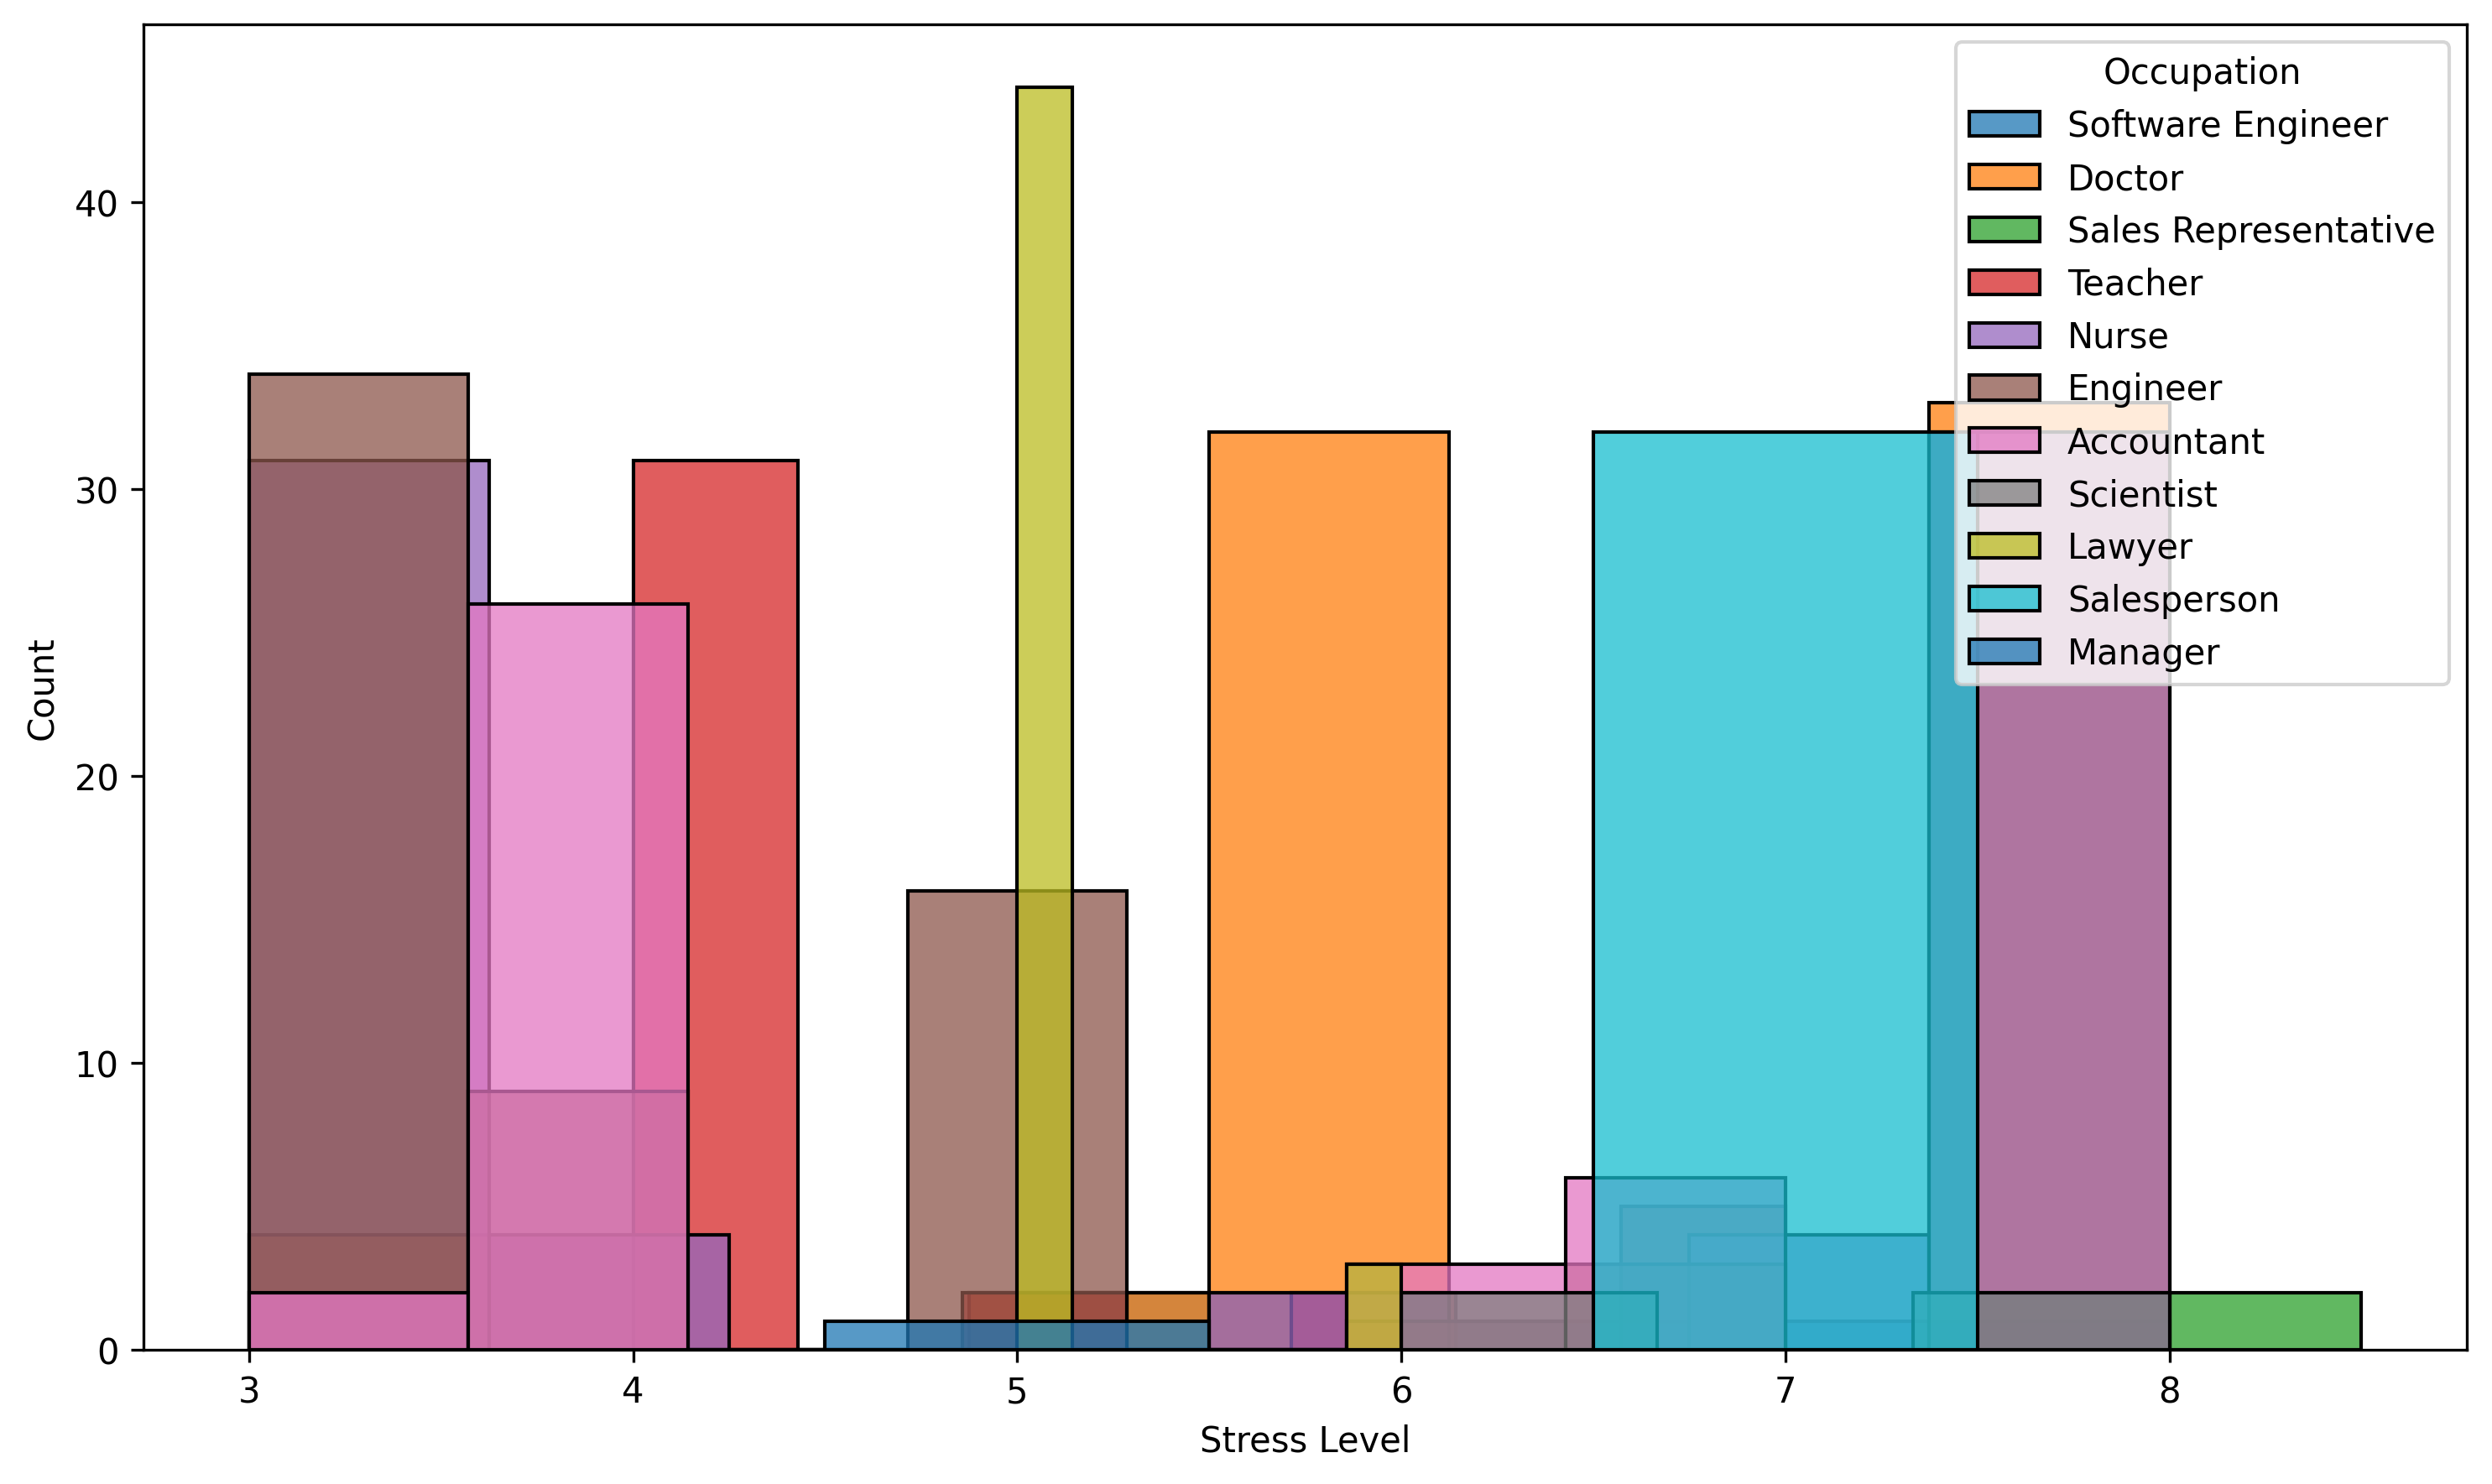
\includegraphics[width=0.8\textwidth]{./images/health_distribution_of_stress_level_for_occupations.png}  % Adjust width as needed
                \caption{Disribution of \textbf{Stress Level} for different \textbf{Occupations}}
                \label{fig:Figure_5}  % Reference the figure using \ref{fig:sample}
    
            \end{figure}
            
            \item Answer based on hypothesis test:
            \textit{If we run ANOVA one-way test, we get results as follows: F-statistic: 21.63598878521177 P-value: 1.355091231304278e-31. So we can say that, the different groups of occupation differ significantly in terms stress level.}
        \end{itemize}

        \item Are different BMI categories significantly different given their blood pres-
        sure? (Hint: Convert blood pressure into two columns and apply your
        test given these new two features.)
        \begin{itemize}
            \item Answer based on hypothesis test (I have divided the Blood Pressure \\ 
            column into two separate columns, Systolic Pressure and Diastolic Pressure.):
            \textit{If we run MANOVA test, we get results represented in Figure~\ref{fig:Figure_6}. Which shows that we have a significant difference between BMI categories in terms of Blood Pressure.}
            
            \begin{figure}[H]  % 'h' means place the figure here

                \centering
                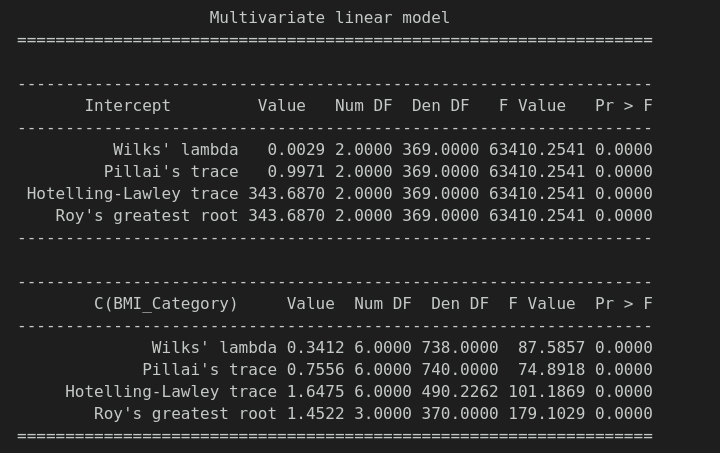
\includegraphics[width=0.8\textwidth]{./images/health_manova_test_for_bp.png}  % Adjust width as needed
                \caption{MANOVA test results for checking significancy of difference between different groups of BMI in terms of their Blood Pressure.}
                \label{fig:Figure_6}  % Reference the figure using \ref{fig:sample}
    
            \end{figure}

        \end{itemize}

        \item Do people with sleep disorders have higher heart rates than those without
        any sleep disorder?
        \begin{itemize}
            \item Answer based on visualization (Figure~\ref{fig:Figure_7}):
            \textit{Yes, based on the plot below we can say that, the people with Sleep Disorder have higher heart rates usually.}
            
            \begin{figure}[H]  % 'h' means place the figure here

                \centering
                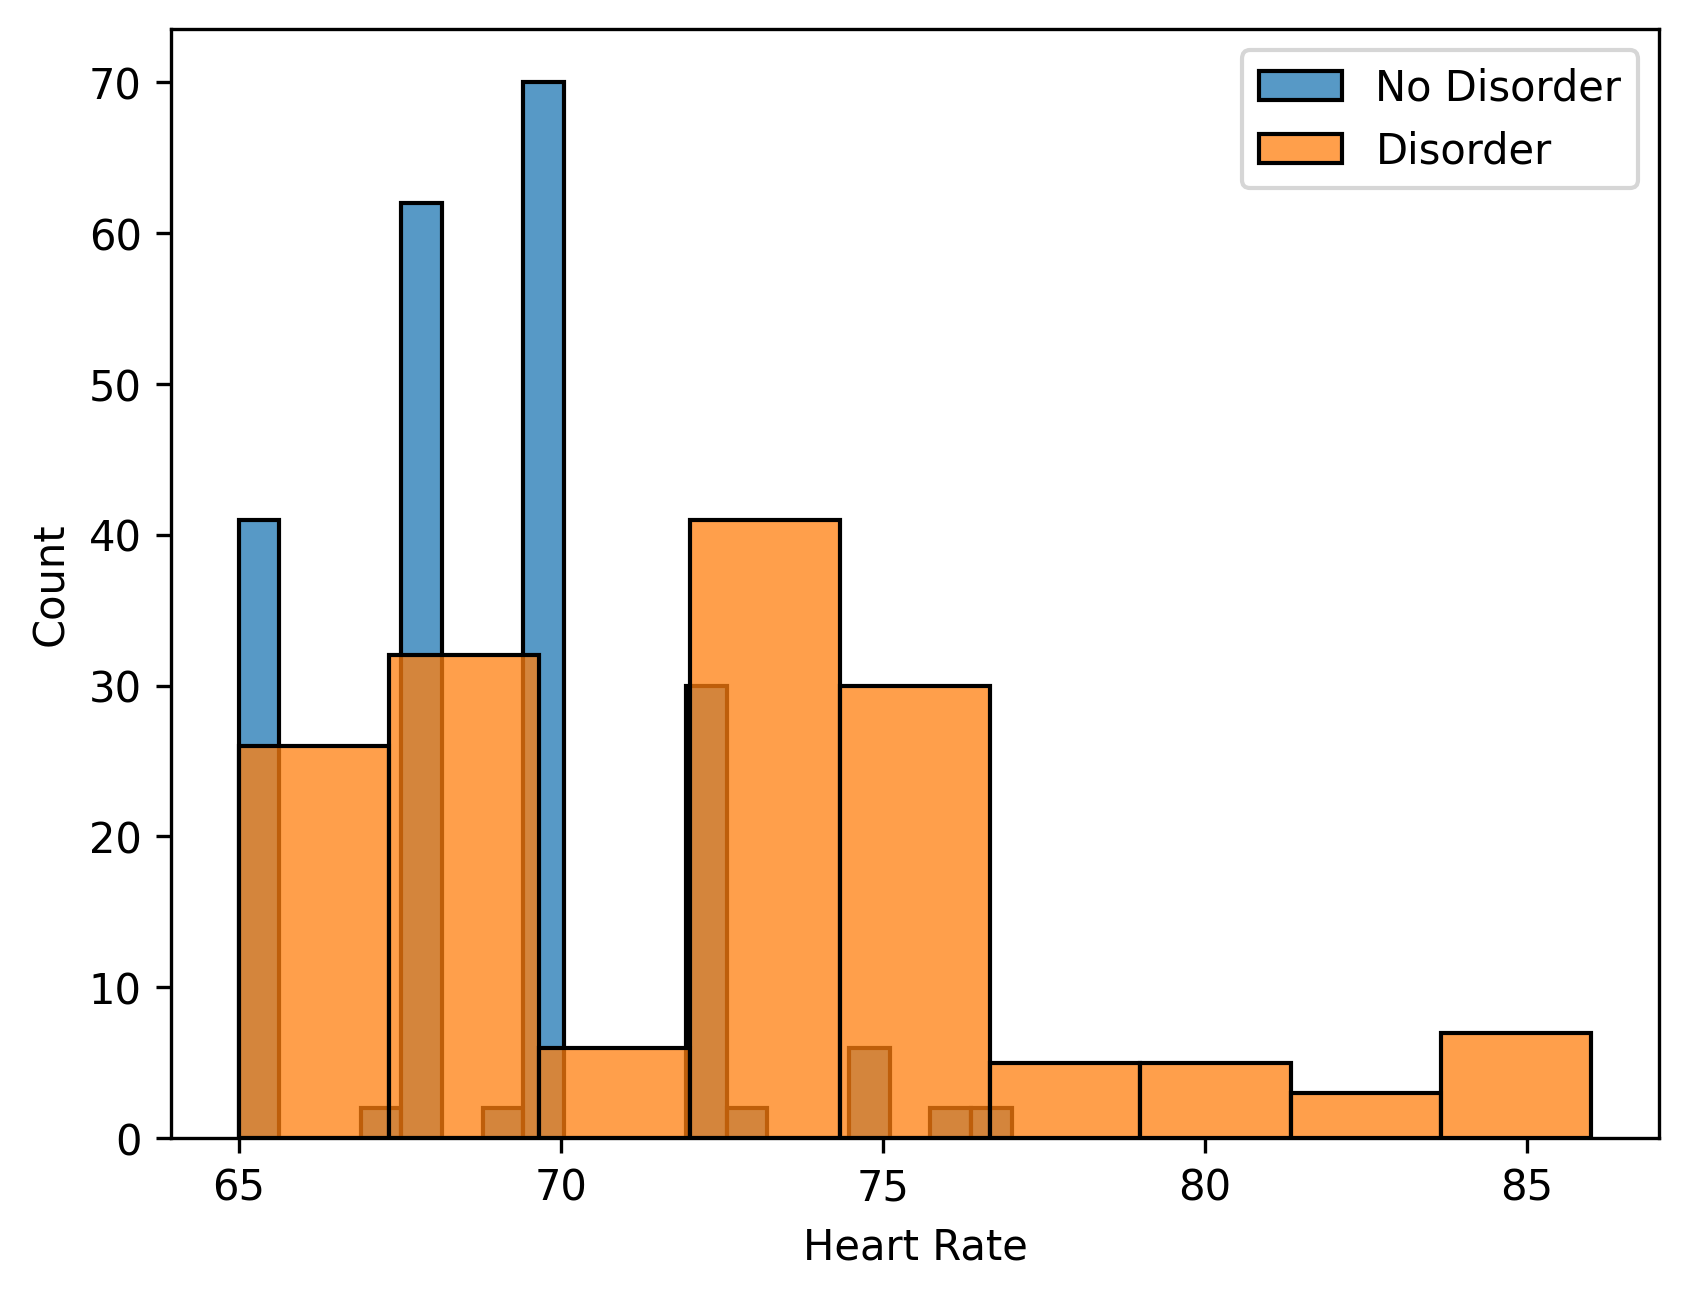
\includegraphics[width=0.8\textwidth]{./images/health_distribution_of_heart_rate_for_people_with_and_without_disorder.png}  % Adjust width as needed
                \caption{Distribution of Heart Rate for two groups, people with and without Sleep Disorder.}
                \label{fig:Figure_7}  % Reference the figure using \ref{fig:sample}
    
            \end{figure}

            \item Answer based on hypothesis test:
            \textit{After performing ANOVA one-way test, we get the following results: F-statistic: 45.5400838475208, P-value: 5.749587721474387e-11, So we can say that, There are significant differences between the groups.}
        \end{itemize}

    \end{enumerate}    

\end{enumerate}

\subsection*{Sleep Health}
\begin{enumerate}
    \item \textbf{Exploratory Data Analysis (EDA)}:
    
    \begin{itemize}

        \item \textbf{Number of rows (data samples) and columns (features) are in the dataset}: (6607, 20)
     
        \item \textbf{Values for each categorical feature}:
        \begin{itemize}

            \item \textbf{Parental\_Involvement}:
            \begin{verbatim}

                ['Low' 'Medium' 'High']

            \end{verbatim}

            \item \textbf{Access\_to\_Resources}:
            \begin{verbatim}

                ['High' 'Medium' 'Low']


            \end{verbatim}

            \item \textbf{Extracurricular\_Activities}:
            \begin{verbatim}

                ['No' 'Yes']

            \end{verbatim}

            \item \textbf{Motivation\_Level}:
            \begin{verbatim}

                ['Low' 'Medium' 'High']

            \end{verbatim}

            \item \textbf{Internet\_Access}:
            \begin{verbatim}

                ['Yes' 'No']

            \end{verbatim}

            \item \textbf{Family\_Income}:
            \begin{verbatim}

                ['Low' 'Medium' 'High']

            \end{verbatim}

            \item \textbf{Teacher\_Quality}:
            \begin{verbatim}

                ['Medium' 'High' 'Low' nan]

            \end{verbatim}

            \item \textbf{School\_Type}:
            \begin{verbatim}

                ['Public' 'Private']

            \end{verbatim}

            \item \textbf{Learning\_Disabilities}:
            \begin{verbatim}

                ['Positive' 'Negative' 'Neutral']

            \end{verbatim}

            \item \textbf{Parental\_Education\_Level}:
            \begin{verbatim}

                ['High School' 'College' 'Postgraduate' nan]

            \end{verbatim}

            \item \textbf{Distance\_from\_Home}:
            \begin{verbatim}

                ['Near' 'Moderate' 'Far' nan]

            \end{verbatim}

            \item \textbf{Gender}:
            \begin{verbatim}

                ['Near' 'Moderate' 'Far' nan]

            \end{verbatim}

        \end{itemize}

        \newpage
        \item \textbf{Description of numerical features}:
        \begin{figure}[H]  % 'h' means place the figure here

            \centering
            \includegraphics[width=0.8\textwidth]{./images/student_distribution_of_numerics.png}  % Adjust width as needed
            \caption{Description of numerical features}
            \label{fig:Figure_8}  % Reference the figure using \ref{fig:sample}
        \end{figure}

        \item \textbf{Datatype of each feature}:
        \begin{verbatim}

            #   Column                      Non-Null Count  Dtype 
            ---  ------                      --------------  ----- 
             0   Hours_Studied               6607 non-null   int64 
             1   Attendance                  6607 non-null   int64 
             2   Parental_Involvement        6607 non-null   object
             3   Access_to_Resources         6607 non-null   object
             4   Extracurricular_Activities  6607 non-null   object
             5   Sleep_Hours                 6607 non-null   int64 
             6   Previous_Scores             6607 non-null   int64 
             7   Motivation_Level            6607 non-null   object
             8   Internet_Access             6607 non-null   object
             9   Tutoring_Sessions           6607 non-null   int64 
             10  Family_Income               6607 non-null   object
             11  Teacher_Quality             6529 non-null   object
             12  School_Type                 6607 non-null   object
             13  Peer_Influence              6607 non-null   object
             14  Physical_Activity           6607 non-null   int64 
             15  Learning_Disabilities       6607 non-null   object
             16  Parental_Education_Level    6517 non-null   object
             17  Distance_from_Home          6540 non-null   object
             18  Gender                      6607 non-null   object
             19  Exam_Score                  6607 non-null   int64 
            dtypes: int64(7), object(13)

        \end{verbatim}

        \item \textbf{Data pre-processing}:
        \begin{itemize}
            
            \item We begin Data pre-processing, by first looking at the distribution of columns for students who have some missing values and those who don't have any.:
            \textit{Based on the distribution of each column, showing on Figure~\ref{fig:Figure_9}, we can see that, the students who don't have any missing values(the blue bars) and the ones who have some missing entries(the yellow ones) are approximately the same. Because the distribution of students who have some missing values is evenly distributed over the whole range of values for the original distribution (distribution of students who don't have any missing values).} 
             
            \begin{figure}[H]  % 'h' means place the figure here

                \centering
                \includegraphics[width=0.8\textwidth]{./images/student_distribution_of_columns.png}  % Adjust width as needed
                \caption{Plot of features for each of the groups (zoom-in)}
                \label{fig:Figure_9}  % Reference the figure using \ref{fig:sample}
    
            \end{figure}

            \item Decission on the rows which have some missing values:
            \textit{Based on the evidences given above, we can say that the students who have some missing values are approximately the same as the ones who don't have any missing entries. So we can simply drop them out of the dataset.}
            
        \end{itemize}

    \end{itemize}

    \item Hypothesis Testing:
    \begin{enumerate}[label= \alph*]
        \item Is Sleep\_Hours correlated with Exam\_Score?
        \textit{If we perform Pearson Correlation Test, we get the following results: Pearson Coefficient: -0.01717144621634847 P-value is: 0.17031732819959972. So we can say that Sleep\_Hours and Exam\_Score are not possibly correlated}
        
        \item Does School\_Type affect Exam\_Score? 
        \textit{If we perform ANOVA one-way test, we get the following results: f\_stat is: 0.7531963873423186, p\_value is: 0.3854987810260675. So we can say that School\_Type doesn't significantly determine Exam\_Score }
       
        \item Does Teacher\_Quality affect Previous\_Scores or Exam\_Score?
        \textit{if we perform MANOVA test, we get the results shown in Figure~\ref{fig:Figure_10}, we can say there, there is a significant differnce in atleast one of the groups. So we perform two ANOVA one-way separate tests to see where is the difference.}
        \begin{figure}[H]  % 'h' means place the figure here

            \centering
            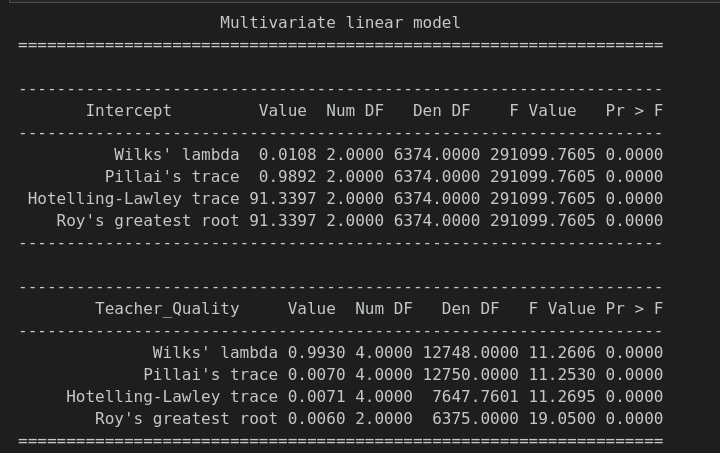
\includegraphics[width=0.8\textwidth]{./images/student_MANOVA_for_teacher_quality.png}  % Adjust width as needed
            \caption{results of MANOVA test for different categories of Teacher\_Quality}
            \label{fig:Figure_10}  % Reference the figure using \ref{fig:sample}

        \end{figure}
        \begin{itemize}
            \item ANOVA one-way test results for Exam\_Score and Teacher\_Quality: F=18.597, p=0.000. So Teacher\_Quality significantly affect Exam\_Score.
            \item ANOVA one-way test results for Previous\_Score and Teacher\_Quality: Previous Score ANOVA: F=3.494, p=0.030 . So Teacher\_Quality significantly affect Previous\_Score.
        \end{itemize}

        \item Do Previous\_Scores influence Exam\_Score? 
        \textit{We perform the Pearson Correlation test and get the following results: Correlation: 0.19111637222616798, p-value is: 1.5821805765966484e-53. Previous\_Scores and Exam\_Score are possibly correlated}

        \item Is Sleep\_Hours normally distributed? 
        \textit{We perform KS test to see whether the distribution of Sleep\_Hours is normal or not. we get the following results: KS Test Statistic: 0.132, p-value: 0.000. So we can say that, Data does not follow a normal distribution}
    
    \end{enumerate}

\end{enumerate}

\end{document}
